\documentclass[12pt,letterpaper]{article}
\usepackage[utf8]{inputenc}
\usepackage[english]{babel}
\usepackage{graphicx}
\usepackage{pdflscape}

\title{\textbf{Department of Computer Science and Engineering}}
\author{\textbf{S.G.Shivanirudh, 185001146}}
\date{29 April 2020}

\begin{document}

\maketitle

\hrule
\section*{\center{UCS1412 - Database Laboratory}}
\hrule 
\bigskip \bigskip

\subsection*{\center{\textbf{Assignment 9: Database Design}}}
\hrule
\bigskip
\subsection*{Part A: Database Design using Normal Forms}
8) TO PROVE DEPENDENCY PRESERVATION PROPERTY:\\
   PERFORM UNION OF ALL FDS IN 3NF RELATIONS AND PROVE IT'S EQUIVALENT TO 1NF LIST OF FDS.\\
\bigskip

Initially we have the following functional dependencies with the 1NF relation \textbf{company},\\
fd1 : \(empid \rightarrow \{name, address, bdate, sex, salary, dno\}\)\\
fd2 : \(dno \rightarrow \{dname, mgr_id\}\)\\
fd3 : \(pno \rightarrow \{pname, pdno\}\)\\
fd4 : \(empid, pno \rightarrow \{hrs\}\)\\

Therefore, the initial list of fds are: \(F = \{fd1, fd2, fd3, fd4\}\)\\

Decomposing the above relation to 3NF, we get the following relations and functional dependencies:\\

\textbf{1. company\_employee}\\
Here,\\ 
Closure of empid : \(\{empid\}^{+} =  \{empid, name, address, bdate, sex, salary, dno\}\)\\
Hence it preserves \textbf{\(empid \rightarrow \{name, address, bdate, sex, salary, dno\}\)}, i.e, fd1.\\
Therefore,  \(F1 = \{ fd1 \}\)\\

\textbf{2.company\_department}\\
Here,\\ 
Closure of dno : \(\{dno\}^{+} =  \{dno, dname, mgr_id\}\)\\
Hence it preserves \textbf{\(dno \rightarrow \{dname, mgr_id\}\)}, i.e, fd2. \\
Therefore,  \(F2 = \{ fd2 \}\)\\

\textbf{3.company\_project}\\
Here,\\ 
Closure of pno : \(\{pno\}^+ =  \{pno, pname, pdno\}\)\\
Hence it preserves \textbf{\(pno \rightarrow \{pname, pdno\}\)}, i.e, fd3. \\
Therefore,  \(F3 = \{ fd3 \}\)\\

\textbf{4.company\_work}\\
Here,\\ 
Closure of \(\{empid, pno\}^+ : \{empid, pno\}^+ =  \{empid, pno, hrs\}\)\\
Hence it preserves \textbf{\(empid, pno \rightarrow \{hrs\}\)} , i.e, fd4.\\
Therefore,  \(F4 = \{ fd4 \}\)\\

\center{Now,\(F1 \cup F2 \cup F3 \cup F4 = \{fd1, fd2, fd3, fd4\} = F\)}

Hence, the functional dependencies are preserved through the decomposition of the 1NF table.
Thus, proved.

\bigskip

\hrule
\bigskip
\newpage
\begin{landscape}
\subsection*{Part B: Database Design using ER diagram}
\bigskip
\flushleft{1) Draw ER diagram for the above requirements. Mention the constraints in the diagram.}\\
\bigskip
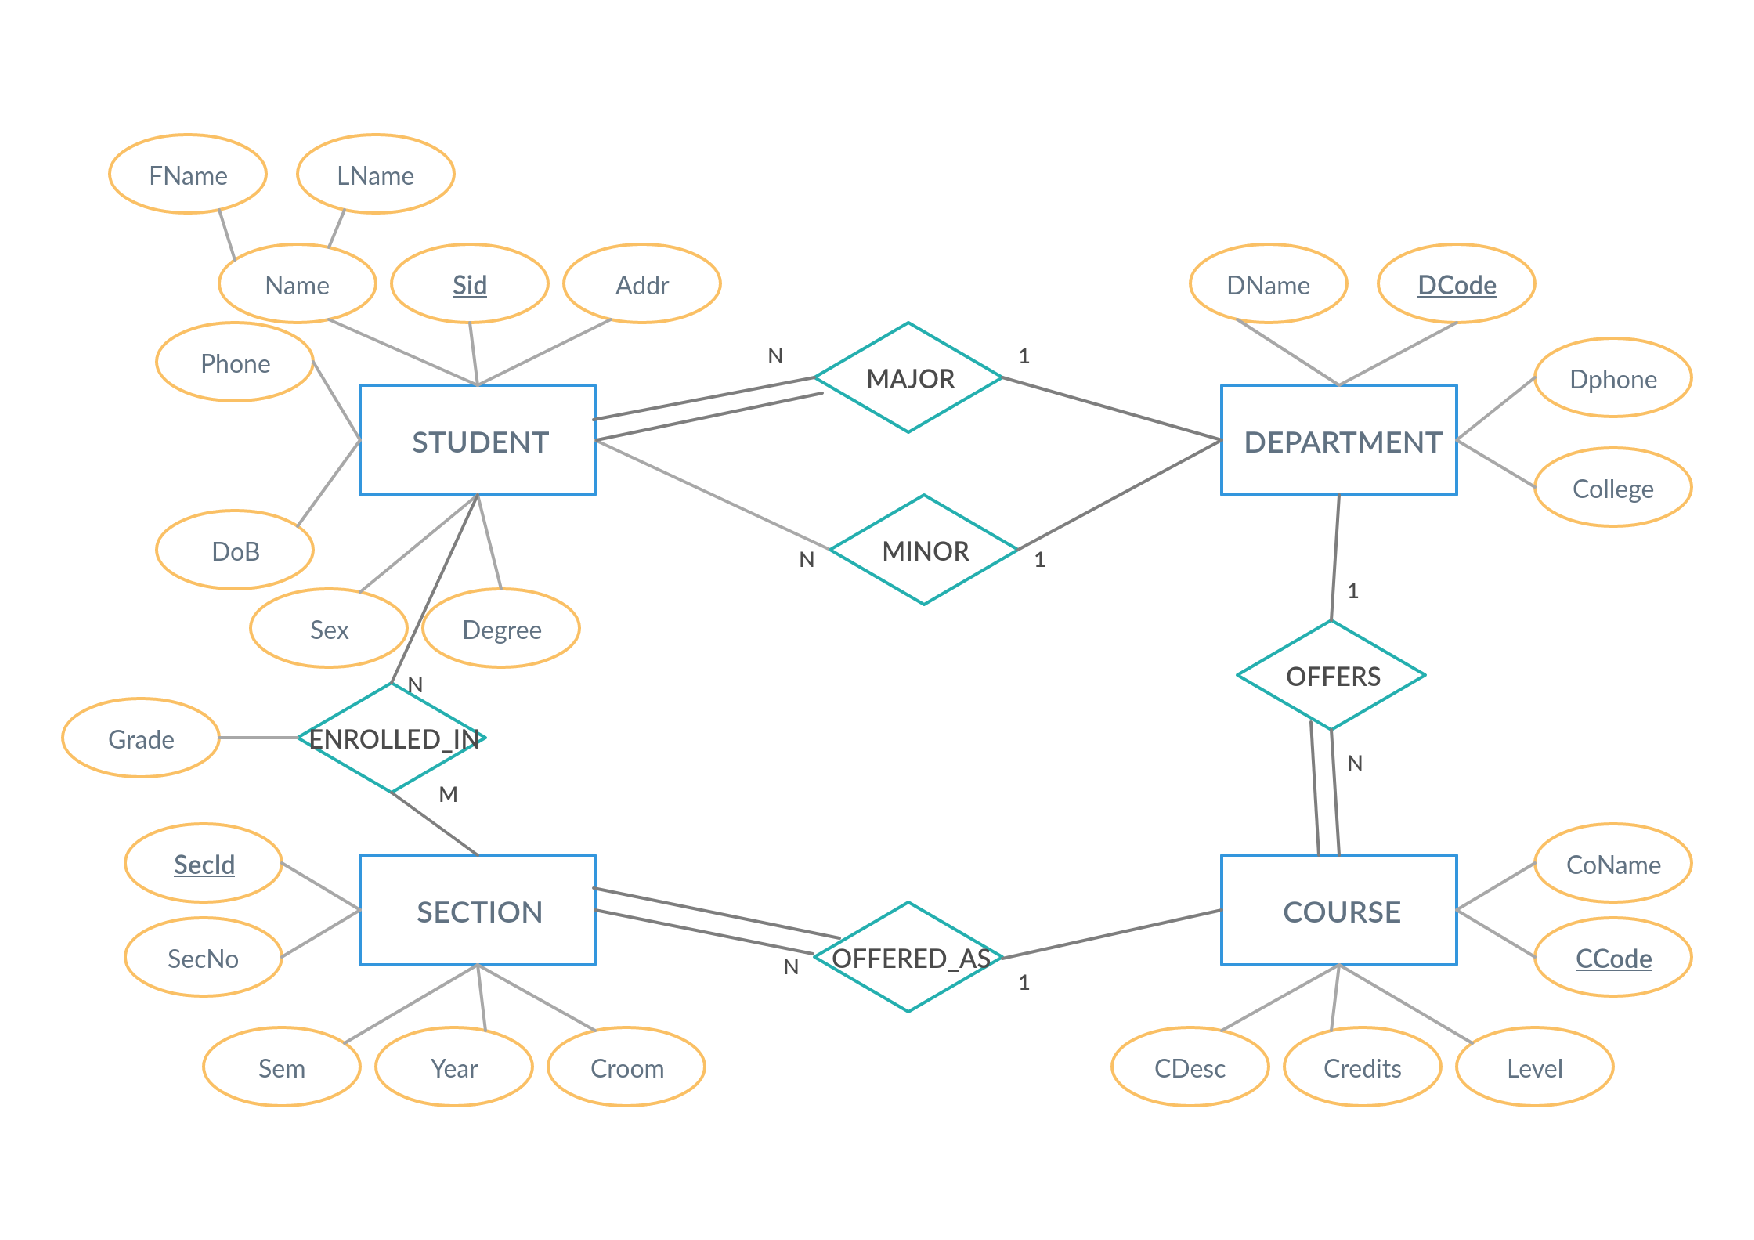
\includegraphics[trim=0mm 20mm 0mm 0mm, clip, width=17.35cm]{ER-converted.pdf}
\bigskip
\newpage
2) Convert the ER into the corresponding relations using ER-Relational Mapping.\\
\bigskip
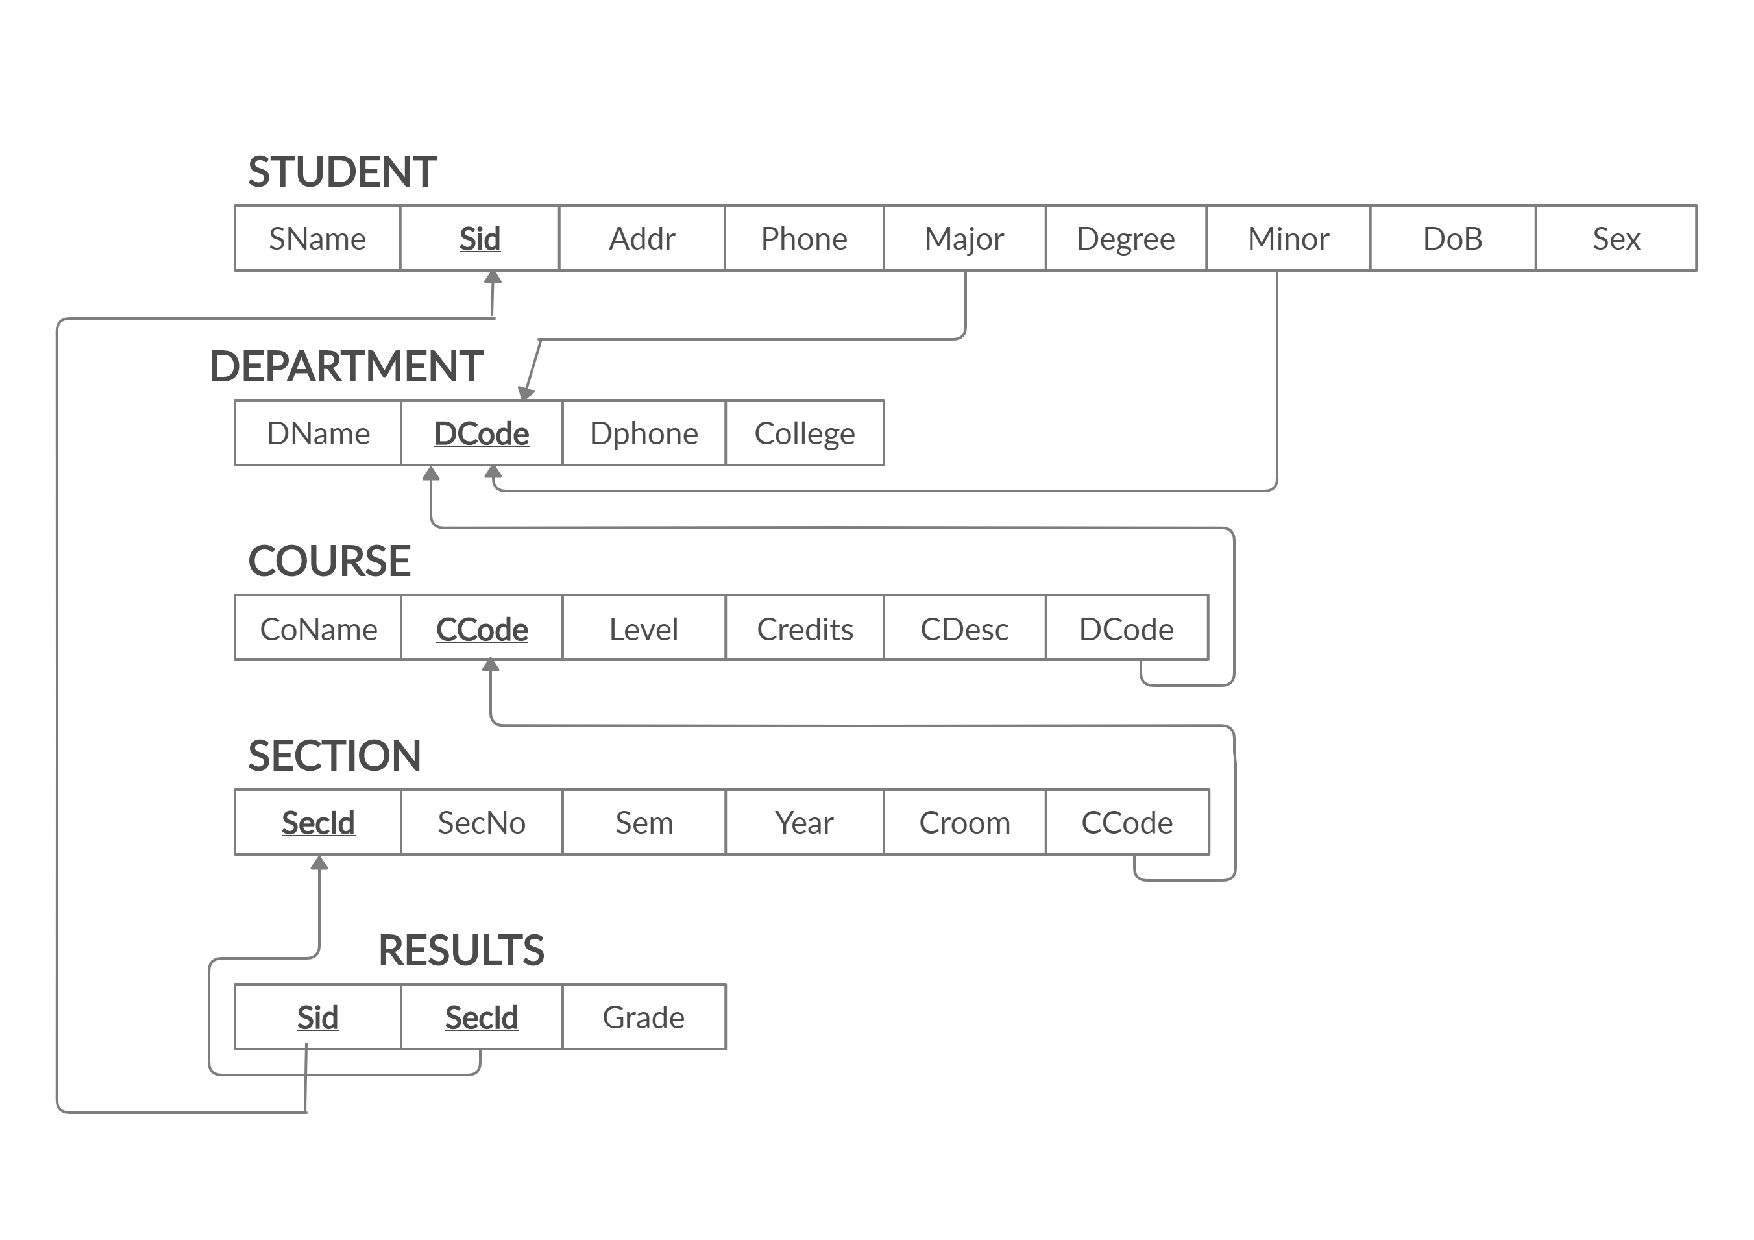
\includegraphics[trim=0mm 20mm 0mm 0mm, clip, width=17.35cm]{Relation-converted.pdf}
\bigskip
\hrule
\end{landscape}
\end{document}